
\chapter{Marco Teórico}

\label{chap2:marco-teorico}

\section{Introducción}

\label{sec21:introduccion}En este capitulo, se resumen las cuatro
áreas principales de estudio relacionados a los sistemas (\emph{Human
Activity Recognition}, \abbr{HAR} ) con miras a definir el problema
del reconocimiento de actividades humanas desde un punto de vista
teórico. La descripción de estas áreas detallan las aplicaciones que
motivan los sistemas \abbr{HAR} y también los mecanismos que llevan
a una implementación factible. 

En la primera sección, se introducen las aplicaciones de contexto
que son el principal marco de trabajo del estudio de sistemas \abbr{HAR}.
En síntesis, nuestro enfoque es detectar las actividades físicas para
dar información de contexto en las acciones diarias de un individuo. 

Las siguientes secciones abarcan todos los elementos requeridos para
implementar los sistemas \abbr{HAR}. Desde el punto de vista de implementación
se discuten los sensores y los teléfonos móviles inteligentes. La
última sección define el marco teórico del reconocimiento de actividades
humanas de acuerdo al estado de arte.

\section{Aplicaciones de contexto}

\label{sec22:contexto}En la actualidad, construir aplicaciones interactivas
requiere que se tenga en cuenta el aspecto del contexto del usuario.
El contexto de un usuario es un medio adicional de interacción entre
humano y computadora, adicional a los otros métodos convencionales
de toma de datos. Este nuevo medio abre nuevas posibilidades de comunicación
y producción de nuevos servicios en computación. 

Pero, ¿qué es el contexto?, citando a otras fuentes podemos definir
el contexto como: 
\begin{quotation}
<<\emph{... cualquier información que pueda ser utilizada para caracterizar
la situación de una entidad. Una entidad es una persona, lugar, u
objeto que es considerado relevante en la interacción entre el usuario
y la aplicación, incluyendo al usuario y la aplicación}>> \cite{Dey2000}. 
\end{quotation}
De manera específica, el contexto de un usuario es el estado acerca
de la información física, emocional o social, sin dejar de lado cualquier
otra situación en la que el usuario esté involucrado y además sea
relevante para la aplicación.

Debido a la libertad de movilidad presentes en la computación móvil
y ubicua, es primordial construir aplicaciones que conozcan el contexto
de sus usuarios, dicho de otro modo aplicaciones de contexto (\emph{context-aware}).
Debido a que el entorno de ejecución cambia con cierto dinamismo,
el rango de situaciones posibles que el usuario experimenta se amplia
y por lo tanto es necesario que los servicios proveídos por una aplicación
se adapten para mejorar la interacción entre el usuario y el computador
\cite{Dey2000}.

Los tipos de contexto prácticos más importantes en las aplicaciones
de contexto con computación móvil son la ubicación, la identidad,
la actividad y el tiempo. Esta caracterización permite a los diseñadores
de aplicaciones escoger el contexto más relevante para su uso.

\section{Sensores}

\label{sec23:sensores} Para resolver el problema del reconocimiento
de actividades humanas uno de los temas a abordar es la recolección
de datos y posiblemente la elección de los sensores utilizados. Se
han utilizando varios sensores para extraer información acerca de
las actividades que un individuo realiza \cite{Chen2012,LaraLabrador2012}.
Los sensores pueden medir signos vitales (ritmo cardíaco, temperatura
del cuerpo, presión arterial), señales de ambiente (intensidad de
luz, temperatura, niveles de sonido, vídeo), movimiento (aceleración,
velocidad), y la ubicación (localización global o en interiores). 

Si clasificamos los sensores con respecto a la disposición de los
mismos en relación a los usuarios, los autores \cite{ReyesOrtiz2015,LaraLabrador2013}
diferencian los mismos entre ambientales, los sensores están ubicados
de manera fija en el entorno que rodea al individuo, y de atuendo
(\emph{wearables}) cuando los sensores están sujetos o anexados al
cuerpo del individuo.

\subsection{Sensores de Ambiente}

Los sensores ambientales, también denominados externos o de entorno,
son un conjunto de dispositivos que se ubican en el entorno y miden
propiedades físicas del mismo, a las personas que rodean, y la interacción
entre los mismos. Existe una amplia variedad de sensores ambientales,
como micrófonos, cámaras de vídeo, sensores de presencia, termómetros
y sensores de profundidad (Ej. el sensor \abbr{Kinect}). 

Varios trabajos exploran el uso de sensores ambientales para el reconocimiento
de actividades humanas y de acciones cotidianas. Entre ellos el expuesto
por \cite{Poppe2007} que realiza un análisis de movimientos humanos
utilizando cámaras de vídeo. En particular, los sistemas basados en
vídeo a pesar de ser bastante efectivos, también deben lidiar con
cuestiones importantes tales como el procesamiento en tiempo real
de la información y la exposición de la privacidad de los usuarios.

\subsection{Sensores de Atuendo}

Los sensores de atuendo (comúnmente denominado\emph{ \abbr{Wearables}})
obtienen señales directamente de los usuarios, estos pueden estar
anexos a varias partes del cuerpo, como la cintura, la muñeca, el
pecho, la pierna y la cabeza \cite{Bao2004}. También pueden formar
parte de alguna vestimenta o estar embebidos en algún accesorio de
uso común como relojes, anteojos y los mismos teléfonos móviles. 

Una característica peculiar de los sensores es su autonomía debido
a la utilización de baterías que proporcionan la energía para operar,
y además pueden operar en conjunto con conexiones inalámbricas (Ej.
\emph{\abbr{Bluetooth}}) para la transmisión de señales. Las señales
obtenidas varían desde la temperatura de la piel, la frecuencia cardíaca,
posicionamiento y hasta el movimiento. Todas estas mediciones son
útiles para tener una constante información del estado de un individuo
en cualquier momento.

Los sensores anexos directamente a un individuo miden señales que
se clasifican comúnmente según los siguientes grupos \cite{LaraLabrador2013}:
\begin{itemize}
\item \textbf{Movimiento}: miden datos inerciales como la aceleración y
la orientación respecto a un marco de referencia relativo al dispositivo
que contiene los sensores. El acelerómetro y el giroscopio son los
más comúnmente utilizados para reconocimiento de actividades con un
bajo consumo de energía y buena precisión de reconocimiento \cite{Bao2004,LaraLabrador2012}.
\item \textbf{Ubicación}: miden datos obtenidos con las redes celulares
de tercera generación (\abbr{3G}) y los satélites de navegación (\emph{Global
Positioning System}, \abbr{GPS}). Provee información de contexto
bastante relevante acerca de la posición del individuo, además de
ciertas medidas de movimiento pero con un consumo moderado de energía.
\item \textbf{Fisiología}: miden signos vitales del individuo como el ritmo
cardíaco (\emph{Heart Rate Monitor},\emph{ }\abbr{HRM}), la temperatura
del cuerpo, el ritmo de respiración, entre otros.
\item \textbf{Ambiente}: miden datos externos que rodean al individuo como
el nivel de ruido, la humedad y/o la temperatura. Los sensores de
luz, cámara, micrófonos y termómetros miden estas señales. 
\end{itemize}
A diferencia de los sensores ubicados fijamente en el ambiente, estos
tienen la ventaja de preservar la privacidad y el área de operación.
La información capturada no es tan sensible como en sensores que capturen
imágenes y vídeo. Además, debido a la miniaturización, los sensores
pueden ser llevados a todas partes por sus usuarios haciéndolos ubicuos,
portables y con cobertura sin limitaciones. Aún así existen desafíos
ha superar como la utilización eficiente de energía y el uso confortable
al estar anexos a una vestimenta sin utilizar cables.

\section{Dispositivos móviles}

\label{sec24:dispositivos-moviles} Desde la aparición de los primeros
teléfonos móviles disponibles en el mercado a principio de los años
ochenta \cite{Tanenbaum2010}, la masificación de uso y producción
de estos dispositivos ha crecido exponencialmente. Se estima que esta
tendencia continuará (cfr. \cite{Ekholm2011}) incluso hasta podría
sobrepasar la población mundial.

Básicamente los teléfonos móviles celulares ofrecen los servicios
de comunicación por voz y datos sin utilizar cables, prácticamente
desde cualquier lugar siempre y cuando esté disponible la cobertura
de red celular. Entre los servicios adicionales podemos destacar el
envío de mensajes de texto (\emph{Short Message Service}, \abbr{SMS})
y multimedia (\emph{Multimedia Messaging Service}, \abbr{MMS}). Debido
a la mejora continua de las capacidades de procesamiento y comunicación,
los usuarios elevaron sus requisitos de acceso a la información de
manera instantánea y sofisticada llevando a la aparición de los teléfonos
móviles inteligentes. 

\subsection{Teléfonos móviles inteligentes}

Los dispositivos móviles, principalmente las últimas generaciones
de teléfonos móviles, en comparación con los móviles convencionales
han incorporado más capacidad de computación (\emph{Central Processing
Unit}, \abbr{CPU}), más \emph{hardware} integrado, servicios y comunicación
inalámbricas. Los teléfonos móviles inteligentes proveen a sus usuarios
mejores características como acceso a la Web, multimedia, juegos,
servicios basados en ubicación, captura de imágenes y vídeos. En la
\tabref{tab2:capacidad-movil} se listan las características comunes
en un teléfono móvil inteligente de gama media.

\begin{table}[htbp]
\centering{}%
\begin{tabular}{|l|p{9cm}|}
\hline 
\textbf{Capacidad}  & \textbf{Elementos} \tabularnewline
\hline 
\hline 
\emph{Hardware}  & \abbr{CPU}, \emph{Graphics Processing Unit}, \abbr{GPU}, Pantalla
táctil, Memoria, Batería\tabularnewline
\hline 
Comunicación  & \abbr{WIFI}, \emph{\abbr{Bluetooth}}, \abbr{3G}/\abbr{4G}\tabularnewline
\hline 
Servicios  & Internet, Aplicaciones\tabularnewline
\hline 
Sensores & Acelerómetro, Giroscopio, Brújula, \abbr{GPS}\tabularnewline
\hline 
\end{tabular}\caption[Capacidades de Teléfonos Modernos]{\label{tab2:capacidad-movil}Capacidades de teléfonos móviles inteligentes}
\end{table}

Tanto los teléfono móviles, como también los reproductores de música
o relojes inteligentes, han incluido desde ya hace un par de años
diversos sensores con miras a enriquecer la experiencia de interacción
humano computador. La utilización de sensores ha propiciado el desarrollo
de aplicaciones que capturan datos medidos de sus usuarios \cite{Lane2010}. 

\section{Aprendizaje Automático}

\label{sec25:aprendizaje-automatico}Una de las técnicas de reconocimiento
de actividades humanas consiste en utilizar un modelo para descubrir
información a partir de los datos en bruto (Ej. señales de movimiento).
Es decir, utilizar algoritmos de aprendizaje automático (\emph{Machine
Learning}, \abbr{ML}) como herramientas para construir, analizar
e inferir actividades por medio de un modelo que utiliza una gran
cantidad de datos medidos con anterioridad acompañados con el comportamiento
observado en los individuos \cite{Chen2012}. Esta técnica involucra
la creación de modelos de clasificación probabilistas o estadísticos,
seguido de los procesos de entrenamiento y aprendizaje.

El aprendizaje automático implica la utilización de datos como conjunto
inicial de entrenamiento para entrenar un algoritmo, uno de muchos
existentes, como redes de Bayes, máquinas de soporte-vector, árboles
de decisión, modelos ocultos de Markov, entre otros \cite{Rajaraman2011}
(véase siguiente sección). Las ventajas de utilizar este enfoque es
la capacidad de manejar incertidumbre e información temporal, pero
su desventaja es que requiere una cantidad grande de datos de entrenamiento,
por lo que puede sufrir de problemas de inicio lento y escasez de
datos. En algunos casos puede no ser escalable y reutilizable porque
un entrenamiento hecho sobre un individuo puede no aplicarse a otro
individuo de distintas características.

\section{Reconocimiento de Actividades Humanas}

El estado del arte de los \abbr{HAR} define las metodologías para
comprender el comportamiento humano a partir de la interpretación
de atributos derivados de fuentes que rodean al individuo \cite{Bao2004,Poppe2007},
por ejemplo el movimiento detectado utilizando sensores, la ubicación
u otras señales fisiológicas. 

El objetivo es identificar las acciones llevadas acabo por una persona
en base a observaciones realizadas sobre el mismo en el entorno en
que se desenvuelve. Las aplicaciones en computación móvil y ubicua
explotan el contexto del usuario haciendo uso de sistemas \abbr{HAR}
como una herramienta tecnológica. Para tener un conocimiento acabado
de este trabajo, en esta sección se expone una descripción general
de aspectos clave como la definición del problema, el proceso de reconocimiento
estándar, las actividades estudiadas y las técnicas de aprendizaje.

\subsection{Definición del Problema}

\label{sec261:definicion-har}De manera a establecer el marco teórico
de estudio del problema \abbr{HAR} en este apartado se describe una
definición formal del problema. Considerando el objetivo y los elementos
de reconocimiento podemos definir el problema como \cite{LaraLabrador2013}:

\begin{definition}[Problema HAR]\label{def2:harp}Dado un conjunto
$S=\{s_{0},...,s_{k-1}\}$ de $k$ series de tiempo, cada una con
una medida particular de cada atributo, y definidas en el intervalo
de tiempo $I=\left[t_{\alpha},t_{\omega}\right]$, el objetivo es
encontrar una partición temporal (\emph{sub}-intervalo de tiempo)
$\left\langle I_{0},...,I_{r-1}\right\rangle $ en $I$, basado en
los datos de $S$ y el conjunto de etiquetas que representan la acción
realizada durante cada intervalo $I_{j}$ (Ej. quieto, caminando,
corriendo, etc.). 

Esto implica que cada intervalo $I_{j}$ son consecutivos, no vacíos,
no superpuestos y que ${\displaystyle \bigcup_{r-1}^{j=0}{I_{j}=I}}$
\end{definition}

Se asumen que las acciones consideradas no pueden ser realizadas simultáneamente,
es decir la persona no realiza la acción de correr y caminar al mismo
tiempo. Además, se debe notar que el problema \abbr{HAR} no es factible
a ser resuelto con una solución determinista. El numero de combinaciones
de valores de atributos y acciones puede ser muy grande, inclusive
infinito; y encontrar los puntos de transición es complejo teniendo
en cuenta que se desconoce la duración de cada acción. 

Es por esta razón que las metodologías de aprendizaje automático son
utilizadas como proceso para reconocer actividades humanas por medio
de la técnica clasificación. Debido a la utilización de aprendizaje
automático para la resolución del problema, se requiere la siguiente
definición relajada del problema \abbr{HAR} descrito anteriormente: 

\begin{definition}[Problema HAR relajado]\label{def2:harp-rel}Dado
(1) un conjunto $W=\{w_{0},...,w_{m-1}\}$ de $m$ ventanas de tiempo
del mismo tamaño, donde cada una está total o parcialmente etiquetada,
y que cada $w_{j}$ contiene un conjunto de series de tiempo $S_{j}=\{s_{j,0},...,s_{j,k-1}\}$
para cada $k$ atributos medidos, y (2) un conjunto $A\text{=}\{\mathrm{a}_{0},...,\mathrm{a}_{n-1}\}$
de etiquetas de actividades, el objetivo es encontrar una función
$f\colon S_{j}\rightarrow A$ que sea evaluada para todos los valores
posibles de $S_{j}$, tal que $f(S_{j})$ es lo más próximo a la acción
realizada durante $w_{j}$ \end{definition}

Considerar la utilización de esta definición relajada introduce un
error en el modelo durante las ventanas de transición entre actividades,
debido a que, en una ventana de tiempo una persona puede estar realizando
más de una acción. Sin embargo, el número de ventanas en transición
es menor al número total de ventanas por lo que el error introducido
por relajar el problema no es significativo para la mayoría de las
aplicaciones.

\subsection{Proceso de Reconocimiento }

\label{sec262:proceso-har}Al igual que en otras aplicaciones de aprendizaje
automático, el proceso de reconocimiento se divide en dos etapas bien
conocidas, la de entrenamiento y las de pruebas (o evaluación).

\begin{figure}[!htbp]
\centering{} 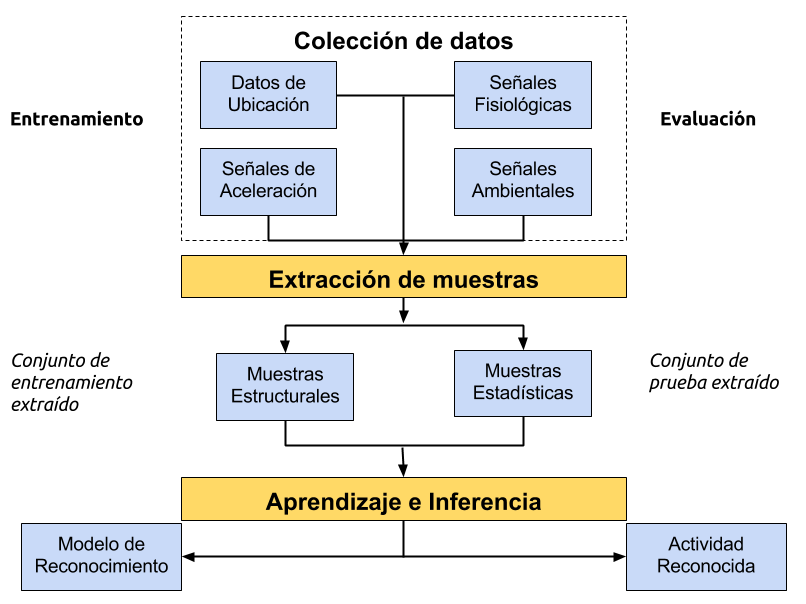
\includegraphics[width=0.7\linewidth]{capitulo-2/graphics/harsystem}
\caption[Flujograma\abbr{HAR}]{\label{fig2:harsystem}Flujo general del Reconocimiento de Actividades
Humanas}
 
\end{figure}

En la \figref{fig2:harsystem} se visualiza las fases comunes de estas
dos etapas \cite{LaraLabrador2013}. La etapa de entrenamiento requiere
inicialmente un conjunto de datos recolectados en una serie de tiempo
con los atributos medidos a partir de individuos que realizan cada
actividad. Las series se dividen en ventanas de tiempo para aplicar
la extracción de muestras filtrando así la información relevante de
las señales en bruto. 

Más adelante, se utilizan métodos de aprendizaje para generar un modelo
de reconocimiento de actividades a partir del conjunto de datos colectado
a través de las características calculadas. Del mismo modo, para la
etapa de prueba o evaluación, se recogen datos durante una ventana
de tiempo, que se utiliza para extraer las mismas características
utilizadas en el modelo, estas se evalúan en el modelo de aprendizaje
previamente entrenado, generando una etiqueta de la actividad predicha.

En las siguientes secciones detallamos las actividades humanas que
son objeto de la clasificación y las funciones de cada etapa.

\subsection{Actividades Humanas}

\label{sec263:actividades-humanas} El diseño e implementación de
un sistema \abbr{HAR} depende totalmente de las actividades que serán
reconocidas. Por lo tanto, el cambio del conjunto de actividades que
un sistema reconoce convierte al problema en uno completamente distinto
lo cual normalmente llega a descartar el diseño original.

Teniendo en cuenta esta razón, y de acuerdo a distintas publicaciones,
presentamos siete grupos distintos de actividades agrupados en la
siguiente \tabref{tab2:grupo-actividades} \cite{LaraLabrador2013}.

\begin{table}[htbp]
\centering{}%
\begin{tabular}{|l|p{9cm}|}
\hline 
\textbf{Grupo}  & \textbf{Actividades} \tabularnewline
\hline 
\hline 
Ambulatoria  & Caminar, correr, sentarse, pararse, quedarse quieto, acostarse, subir
escaleras, descender escaleras, usar escaleras mecánicas, usar elevador.\tabularnewline
\hline 
Transporte  & Andar en bus, bicicleta y conducir \tabularnewline
\hline 
En el teléfono  & Enviar mensajes de texto y hacer llamadas \tabularnewline
\hline 
Actividades diarias  & Comer, beber, trabajar en la PC, observar TV, leer un libro, cepillarse
los dientes, aspirar el piso, y otros. \tabularnewline
\hline 
Ejercitarse  & Alzar pesas, bicicleta estática, remo y otros. \tabularnewline
\hline 
Militares  & Arrastrarse, en cuclillas, abrir la puerta \tabularnewline
\hline 
Parte superior del cuerpo  & Masticar, hablar, mover la cabeza, tragar líquidos, mirar. \tabularnewline
\hline 
\end{tabular}\caption[Grupos de Actividades]{\label{tab2:grupo-actividades}Grupos de Actividades}
\end{table}

Las actividades pueden separase en varios grupos de acuerdo a la duración
y la complejidad del evento. Los eventos cortos son movimientos de
transición y movimientos en base a gestos. Los eventos al que nos
enfocamos en este trabajo son aquellos que se componen de las actividades
básicas de larga duración que se caracterizan por las acciones continuas
y cíclicas de un individuo \cite{ReyesOrtiz2015}. El estudio en este
trabajo no se basa en actividades complejas que sean una secuencia
de actividades básicas y eventos cortos.

Se define como objetivo de estudio la detección de actividades básicas
ambulatorias y de transporte, de larga duración y sin cambios bruscos
de transición.

\subsection{Colección de Datos}

La definición del método de colección de datos es un punto importante
en un sistema \abbr{HAR}. Según como se realiza la observación del
individuo, puede darse el caso de captura en ambientes realistas los
cuales son los ideales pero no siempre posibles, y también los ambientes
casi-realistas llevadas acabo en laboratorios donde se simula así
las condiciones reales de las actividades humanas. Por otro lado tenemos
los ambientes totalmente controlados en laboratorio.

Una falla en el diseño de un sistema \abbr{HAR} se puede dar por
no considerar las condiciones reales de las actividades, tales como
actividades no tenidas en cuenta, calibración de sensores, ruido,
etc. Otra de las consideraciones a tener en cuenta en este punto es
la cantidad de individuos para realizar la colección, es recomendable
el mayor cantidad de individuos en distintos tipos de edades y condiciones
físicas.

\subsection{Extracción de Muestras}

Para cualquier problema de aprendizaje automático, la selección de
características se refiere al proceso de selección de un conjunto
significativo de características que aporten relevancia a la capacidad
de discriminación en un algoritmo de aprendizaje. Por otro lado, la
extracción de características, tiene como objetivo disminuir la cantidad
de características a utilizar mediante distintas transformaciones
entre ellas para obtener nuevas características reducidas sin perder
información relevante del conjunto de datos originales. La selección
y extracción de características también permite reducir los tiempos
de procesamiento en la fase de entrenamiento y aumenta el rendimiento
en la fase de evaluación

Dependiendo de la aplicación, las características requeridas para
la extracción de la información relevante pueden variar. En el caso
particular de \abbr{HAR}, una representación reducida de los datos
del sensor se puede utilizar como la entrada del algoritmo de reconocimiento.
Esto se logra mediante medición de la señal del sensor en varios dominios,
pudiendo ser en tiempo y frecuencia.

\subsection{Aprendizaje e Inferencia}

Varios enfoques de aprendizaje automático se han desarrollado a lo
largo de los años para resolver el problema de \abbr{HAR}. En su
mayoría a través de algoritmos de aprendizaje supervisado aunque también
se han propuesto métodos semisupervisados y no supervisados.

La diferencia entre el aprendizaje supervisado y no supervisado consiste
en la utilización de datos etiquetados y no etiquetados respectivamente.
Debido a que el objetivo de un sistema \abbr{HAR} es encontrar una
actividad etiquetada como caminando, corriendo, quieto, etc., la mayoría
de los sistemas \abbr{HAR} utilizan un enfoque supervisado.

El aprendizaje automático supervisado, referido como clasificación
para problemas de clases discretas, ha sido un área bastante estudiada
con varios algoritmos propuestos, algunos de los cuales son citados
en la \tabref{tab2:metodos-aprendizaje} \cite{James2013}. Estas
técnicas resuelven otras tareas además de la clasificación como la
regresión y el agrupamiento.

\begin{table}[tbph]
\begin{centering}
\begin{tabular}{|>{\raggedright}m{4cm}|>{\raggedright}p{9cm}|}
\hline 
\textbf{Grupo}  & \textbf{Actividades} \tabularnewline
\hline 
\hline 
Basados en Reglas & Árboles de decisión (\emph{Decision Tree}, \abbr{DT})

Selvas aleatorias (\emph{Random Forest}, \abbr{RF})\tabularnewline
\hline 
Enfoques Geométricos  & Vecinos próximos (\emph{k-Nearest Neighbors}, \abbr{k-NN})

Redes neuronales (\emph{Artificial Neural Networks}, \abbr{ANN})

Máquinas de soporte-vector (\emph{Support-Vector Machine}, \abbr{SVM})\tabularnewline
\hline 
Clasificación Probabilista & Clasificadores de Bayes (\emph{Naive Bayes}, \abbr{NB}), 

Modelos ocultos de Markov (\emph{Hidden Markov Models}, \abbr{HMM})\tabularnewline
\hline 
\end{tabular}
\par\end{centering}
\caption[Métodos de aprendizaje agrupados]{\label{tab2:metodos-aprendizaje}Resumen de métodos de aprendizaje
agrupados por tipo}
\end{table}

Algunos aspectos relevantes para la selección de un algoritmo de aprendizaje
pueden ser: el consumo de energía, los requisitos de memoria, la complejidad
de computo e interpretación, entre otros. Estos aspectos se agudizan
si se utilizan dispositivos móviles inteligentes. Por ejemplo, los
árboles de decisión podría ser el método preferido cuando se requiere
simplicidad en la implementación, mientras que los métodos \abbr{SVM}
para aplicaciones que requieran un alto rendimiento pero con mayor
complejidad \cite{ReyesOrtiz2015}.

En el capitulo \ref{chap:Aprendizaje-Automatico} se detalla la base
teórica referente a las técnicas de aprendizaje automático supervisados
y el método de árboles de decisión electo para este trabajo.
